\documentclass[tikz,border=5pt]{standalone}

\begin{document}
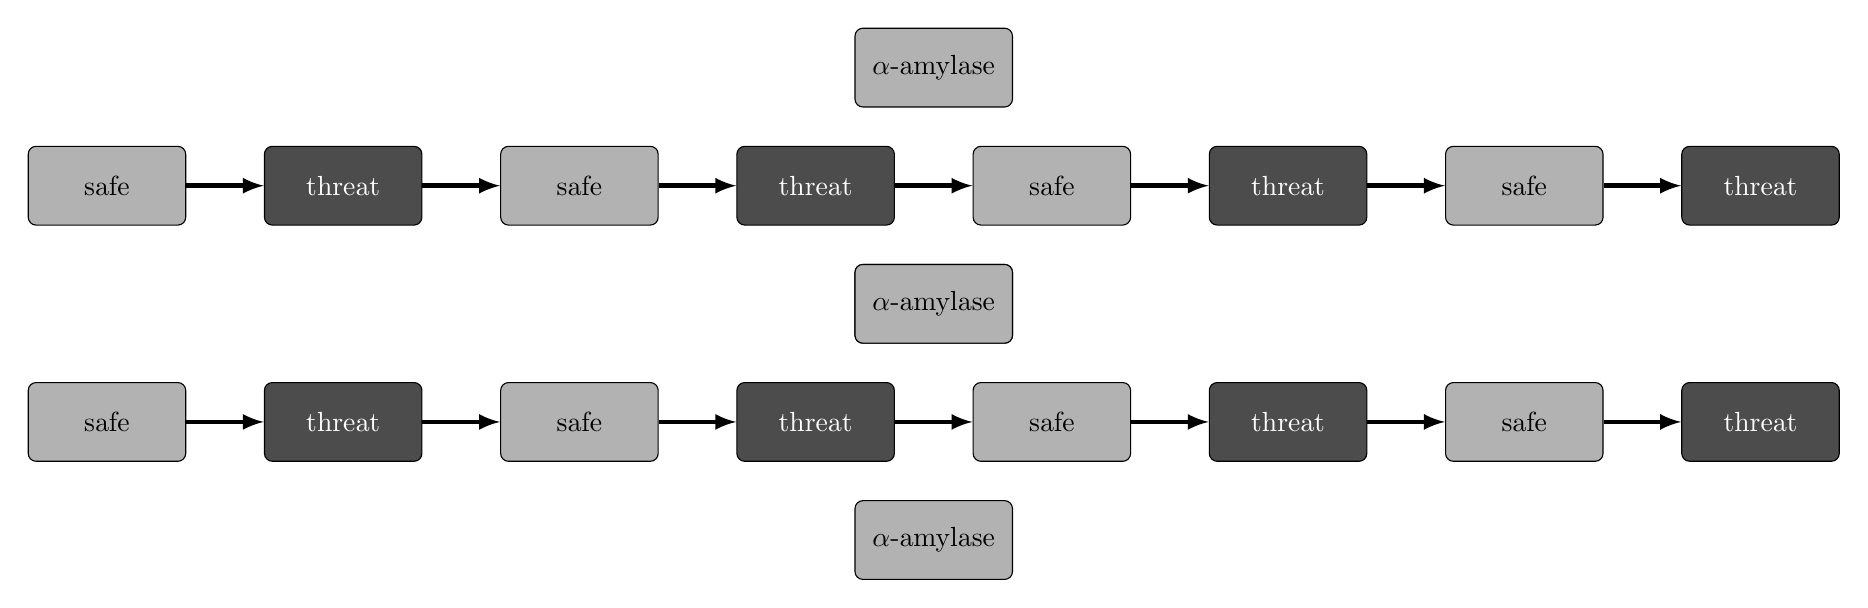
\begin{tikzpicture}[xscale=1, yscale=1]
	\tikzstyle{arrow}=[draw, -latex]
	\newcommand\Xmax{5}
	\newcommand\XMid{\Xmax/2}
	\newcommand\Xtext{\Xmax}

	\newcommand\YSpace{1}
	\newcommand\Yclass{1.5}
	\newcommand\YStim{\Yclass-\YSpace}
	\newcommand\Yxs{\YStim-\YSpace}
	\newcommand\XStart{0}

	\draw [rounded corners=1mm,fill=black!30] (10.5, 1.5) rectangle (12.5,2.5)  node [midway, minimum width=2cm] (AA3) {$\alpha$-amylase};
\foreach \j in {0,...,1}
{
\pgfmathtruncatemacro{\YS}{(\j * -3) };
\pgfmathtruncatemacro{\YF}{(\YS + 1)};
	\foreach \i in {1,...,4}
	{
			\pgfmathtruncatemacro{\IndexS}{(\i * 2) + (\j * 9)};
			\pgfmathtruncatemacro{\IndexF}{(\IndexS) - 1};
	        \pgfmathtruncatemacro{\StartF}{((\i - 1)  * 6)};
	        \pgfmathtruncatemacro{\StartS}{\StartF  + 6 / 2};
			\draw [rounded corners=1mm,fill=black!30] (\StartF,\YS) rectangle (\StartF+2,\YF)  node [midway, minimum width=2cm] (\IndexF) {safe};
			\draw [rounded corners=1mm,fill=black!70] (\StartS,\YS) rectangle (\StartS+2,\YF)  node [midway, text = white, minimum width=2cm] (\IndexS) {threat};

	}
	\draw [rounded corners=1mm,fill=black!30] (10.5, -1.5) rectangle (12.5,-.5)  node [midway, minimum width=2cm] (AA2) {$\alpha$-amylase};
}

	\draw [rounded corners=1mm,fill=black!30] (10.5, -4.5) rectangle (12.5,-3.5)  node [midway, minimum width=2cm] (AA3) {$\alpha$-amylase};

\foreach \j in {0,...,1}
{
	\foreach \i in {1,...,7}
	{
			\pgfmathtruncatemacro{\current}{(\i) + (\j * 9)};
			\pgfmathtruncatemacro{\next}{(\current) + 1};
			\path [arrow, ultra thick] (\current.east) -- (\next.west);
	}
}





	 %      \draw [rounded corners=1mm] (\XStart,0) rectangle (\XStart+2,1)  node (rect) {};
	 % \renewcommand\XStart{\XStart\XSep}
	 % \draw [rounded corners=1mm] (\XStart,0) rectangle (\XStart+2,1)  node (rect1) {};
	 % \renewcommand\XStart{\XStart\XSep}
	 %  \node[rounded corners=3pt, draw, fill=black!30] at (0, 0) () {Hallo!};
	 %  \node[rectangle, rounded corners=3pt, draw, fill=black!70] at (2, 0) () {Hallo!};
	 %

	 
	%  % Stimulus
	%
	% \node [draw, circle, minimum width=1cm, ultra thick] at (\XMid,\YStim) (mu) {$\mu$};
	% \node [anchor=west, align=left] at (\Xtext, \YStim) (Cstat) {$p(\mu) = \mathcal{N}(\mu;0,\sigma_{\mu}^2)$};
	%
	%  % Observations
	% \node [draw, circle, minimum width=1cm, ultra thick] at (.5,\Yxs) (x0) {$\delta x_0$};
	% \node [draw, circle, minimum width=1cm, ultra thick] at (1.5,\Yxs) (x1) {$\delta x_1$};
	% \node [draw, circle, minimum width=1cm, ultra thick] at (2.5,\Yxs) (x2) {$\delta x_2$};
	% \node [draw, circle, minimum width=1cm, ultra thick, white] at (3.5,\Yxs) (dots) {\textcolor{black}{$\ldots$}};
	% \node [draw, circle, minimum width=1cm, ultra thick] at (4.5,\Yxs) (xt) {$\delta x_t$};
	%
	%
	%  % Path Arrows
	% % \path [arrow, ultra thick] (C) -- (S);
	%
	% \path [arrow, ultra thick] (mu) -- (x0.north);
	% \path [arrow, ultra thick] (mu) -- (x1.north);
	% \path [arrow, ultra thick] (mu) -- (x2.north);
	% \path [arrow, ultra thick] (mu) -- (dots.north);
	% \path [arrow, ultra thick] (mu) -- (xt.north);

\end{tikzpicture}


\end{document}

